\newpage

\section{Introduction}
Low birth weight (LBW) is defined by the World Health Organisation as a birth of an infant weighing less than 2500 grams. Low birth weight is closely associated with fetal and perinatal mortality, inhibited growth and cognitive development, and chronic diseases later in life. Physicians are therefore interested in understanding the effects of different behavioural and environmental variables on the likelihood of having a low birth weight.

The variables identified in table \ref{tab:variables} have been shown to be associated with low birth weight in the obstetrical literature. The goal of this study is to ascertain if these variables were important in the population being served in the medical center where this data was collected. We then build, compare, and discuss different models for predicting the likelihood of a low weight birth given these variables. 

\vspace{0.3cm}
\renewcommand\arraystretch{1.2}
\begin{table}[ht]
\centering
\begin{tabular}[t]{ll}
\toprule
Variable & Abbreviation \\
\midrule
Low Birth Weight (0 or 1) & LOW \\
Age of the Mother in Years & AGE \\
Weight in pounds at the last menstrual period & LWT \\
Race (1 - White, 2 = Black, 3 = Other) & RACE \\
Smoking status during pregnancy (Yes = 1, No = 0) & SMOKE \\
Number of previous premature labours & PTL \\
History of hypertension & HT \\
Presence of uterine irritability & UI \\
Number of visits to physician during first trimester & FTV \\
Birth weight in grams & BWT \\
\bottomrule
\end{tabular}
\caption{Caption below table.}
\label{tab:variables}
\end{table}%

\section{Review of the Obstetrical Literature}
Reviewing the obstetrical literature allows us to understand how these variables and their interactions should influence the likelihood of a low birth weight. This information can then be compared with the results from an exploratory analysis of the data (see Section \ref{exploratory}), allowing us to determine how the data differs from what would be expected and to make informed decisions when building predictive models.

\subsection{Effects of variables on low birth weight}
A brief description of the effect of each variable on low birth weight is given below.
\begin{itemize}
    \item \textbf{AGE -} Fraser and Brockert [1995] showed that teenage mothers have a significantly higher risk than mothers who were 20 to 24 years of age of delivering an infant who had low birth weight.\cite{AgeYoung} However, advancing maternal age is associated with a decreased potential for fetal growth and it has been shown that the adjusted risk for low birth weight at term is the lowest in younger mothers and increases with advancing maternal age.\cite{MaternalAge}
    
    \item \textbf{SMOKE -}
    Smoking during pregnancy inhibits full fetal development and is closely associated with low birth weight.\cite{SmokeLBW} However, the degree to which smoking affects low birth weight varies significantly with the average number of cigarettes smoked per day, with birth weight decreasing as the category of cigarette number per day increases.\cite{SmokeReduction} This study uses a binary SMOKE variable - a more detailed categorisation of smokers would most likely improve the quality of the models.
    
    \item \textbf{RACE -}
    There is a higher rate of LBW among black women when compared with white women.\cite{RaceDifference} Race effectively acts as a proxy variable - encoding information about sociodemographic, health-related, and behavioural differences between different racial groups.\cite{RaceLBW}
    
    \item \textbf{LWT -}
    Progressive increase in pre-pregnancy weight was paralleled by progressive increase in mean birth weight and decrease in the incidence of low weight births.\cite{Weight}
    
    \item \textbf{PTL -}
    The risk of the birth of a subsequent low birth weight infant is 2 to 5 times higher than average for mothers who have had a previous low birth weight delivery and increases with the number of prior low-weight births.\cite{bakketeig1979tendency}
    
    \item \textbf{HT -}
    Both chronic and pregnancy induced hypertension are strongly associated with retarded fetal growth and pre-term birth. As a result, maternal hypertension is strongly associated with low infant birth weight. \cite{InducedHT}\cite{HTRace}
    
    \item \textbf{FTV -}
    Increasing the number of physician visits can lead to earlier and more accurate diagnosis of LBW risk factors. Many studies have established a link between date of the first visit, total number of visits and length of pregnancy and LBW, a relation that is stronger if the first visit is delayed or if the number of visits is smaller than normal.\cite{FTV1}\cite{FTV2}\cite{FTV3}
    
    \item \textbf{UI -}
    The incidence of preterm labour in women with uterine irritability is not as frequent as in patients with other high-risk factors. However, preterm labour does occur in patients with uterine irritability at a rate higher than that in the general obstetric population.\cite{UI}
    
    
\end{itemize}

\subsection{Interactions between variables}\label{literatureInterations}
An interaction describes a situation in which the effect of one non-dependent variable on 'LOW' is dependant on the state of a second non-dependent variable. This is equivalent to saying the effects of the the non-dependent variables are not additive. Listed below are the interactions which are most relevant according to the obstetrical literature.

\begin{itemize}
    \item \textbf{SMOKE/AGE -}
    Older mothers, who are already at risk of giving birth to low birth weight infants, might be more susceptible to the effects of maternal smoking. [reference] determined that maternal age has a modifying effect on the association between maternal smoking and birth weight. The association between low birth weight and age increases with maternal age.\cite{SmokeAge}
    
    \item \textbf{SMOKE/RACE -}
    The LBW risk difference associated with smoking is greater among black women. This might be due to the fact that even if black women smoked significantly fewer cigarettes per day, they might have higher cotinine levels compared to white women. \cite{SmokeRace}
    
    \item \textbf{AGE/FTV -}
    For adult first-time mothers, fewer than 10 prenatal care visits was the only significant factor affecting LBW. Therefore, health education programs or prenatal care aimed at preventing LBW should be tailored according to the age of pregnant mothers. The effect of FTV on LBW is stronger for younger mothers.\cite{AgeFTV}
\end{itemize}

\section{Structure of the Dataset}
The dataset in question contains data collected on 189 women, 59 of which had low birth weight babies and 130 of which had normal birth weight babies. In this study, there is a single binary response variable "LOW", where

\begin{equation*}
    \text{LOW}=
    \begin{cases}
      1, & \text{if}\ \text{Birth weight} < 2500\text{g} \\
      0, & \text{otherwise}
    \end{cases}
\end{equation*}

 The eight covariates provided were treated as either categorical or continuous variables in the conducted analyses. Maternal age (AGE), maternal weight (LTW), number of physician visits during the first trimester (FTV), and history of premature labour (PTL) were analysed as continuous variables. It should be noted that FTV and PTL are in reality discrete quantitative variables, as they are numeric variables with a countable (i.e. not infinite) number of values. However, because these covariates have numerous levels which have a defined “order” to them, the decision was made to treat them as continuous predictors in the regression model. Maternal race (RACE), smoking status (SMOKE), history of hypertension (HT), and presence of uterine irritability (UI) were treated as categorical variables.

\section{Exploratory Analysis}\label{exploratory}
An exploratory analysis is performed, first investigating the correlation between the predictor variables and the response variable, and then checking for meaningful interactions between predictor variables. The reasons for these analyses are twofold:
\begin{itemize}
    \item Investigate whether the associations and correlations in our data are consistent with the obstetrical literature.
    \item As a guideline for the inclusion of main effects and interactions in candidate models.
\end{itemize}

Note that when calculating correlation, no inferences are made about causality. Instead it is used to compare the associations in the data with those in the obstetrical literature to see if the data is consistent. Also a significant correlation with low birth weight gives reason to strongly consider these variables as main effects in the candidate models.

\subsection{Correlation with LBW}
The Spearman correlation coefficient was calculated between the dependant variable (BWT) and each of the continuous variables - AGE, LWT, FTV, and PTL. The Spearman correlation was chosen due to the non-normal distribution of each of these variables, as determined by a series of Shapiro-Wilks tests. The Spearman correlation coefficients and related p-values are given in table \ref{tab:Spearman}. Both LWT and PTL are significantly correlated with BWT, with p-values of 0.001 and 0.005 respectively. They are therefore strong candidates to consider as parameters in the candidate models.

\vspace{0.3cm}
\renewcommand\arraystretch{1.2}
\begin{table}[ht]
\centering
\begin{tabular}[t]{lllll}
\toprule
& AGE & LWT & FTV & PTL \\
\midrule
$\rho$ & 0.061 & 0.248 & 0.07 & -0.204 \\
p-value & 0.404 & 0.001 & 0.338 & 0.005 \\
\bottomrule
\end{tabular}
\captionsetup{width=.69\linewidth}
\caption{Spearman correlation results and their respective p-values. The highlighted cells indicate statistically significant results.}
\label{tab:Spearman}
\end{table}%

Box plots were used to identify how the non-continuous variables in the dataset were associated with birth weight and are therefore strong candidates to consider as parameters in the candidate models (see section \ref{BuildingOne} and section \ref{BuildingTwo}).

\vspace{0.5cm}
\begin{figure}[!htb]
        \centering
        \begin{subfigure}[b]{0.4\textwidth}
            \centering
            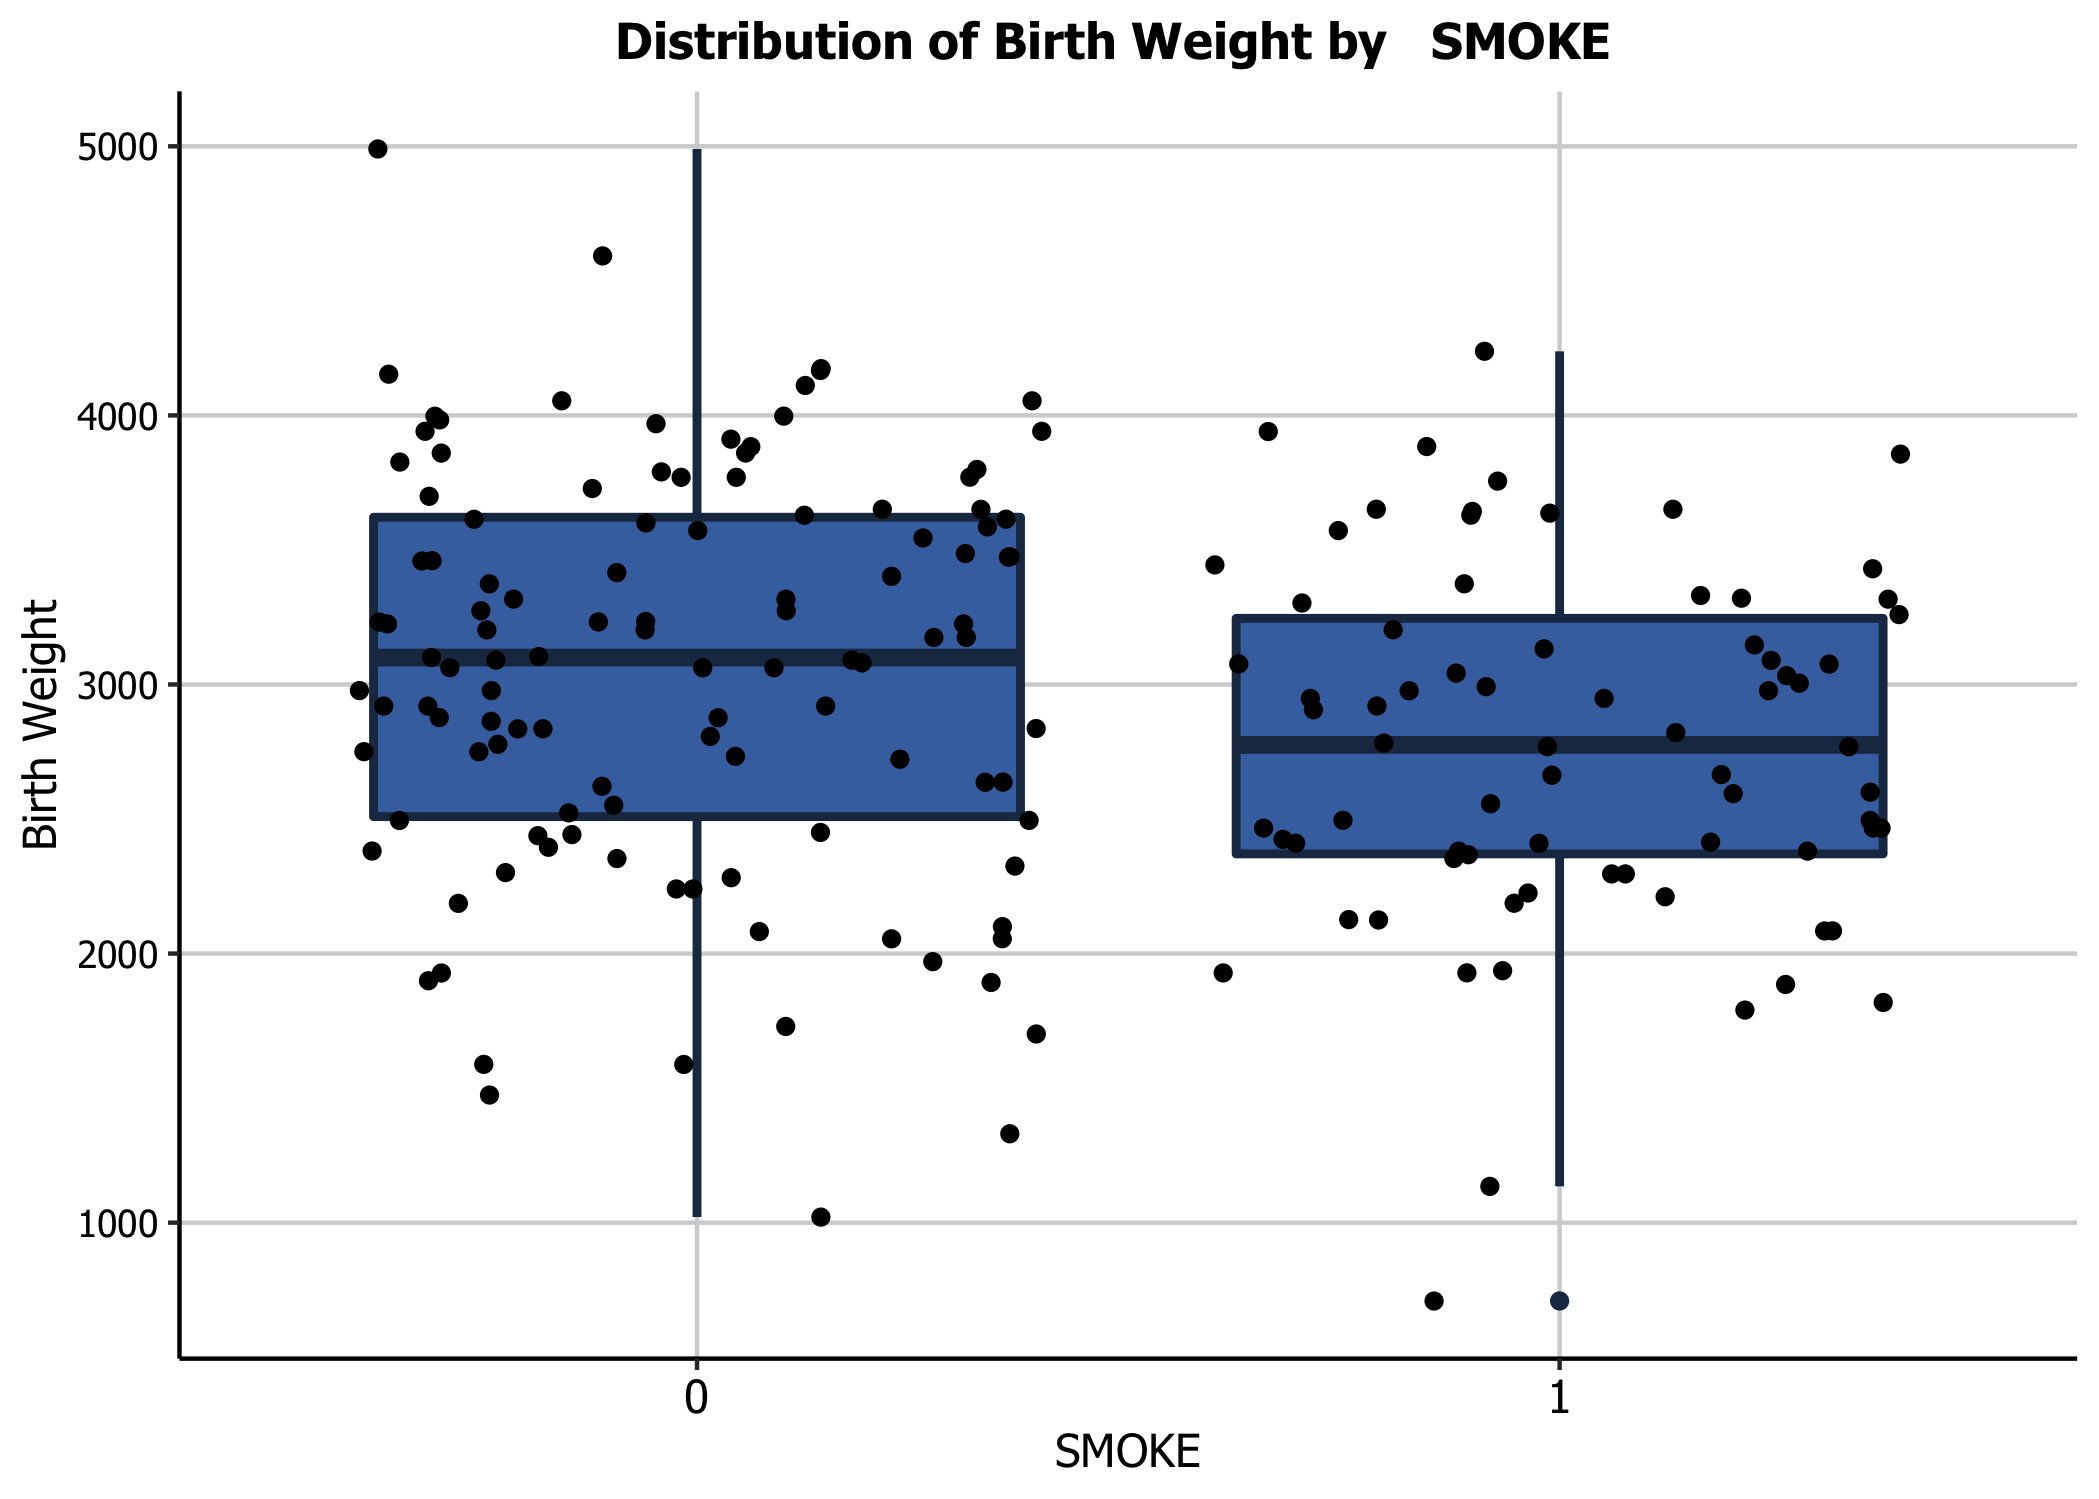
\includegraphics[width=\textwidth]{Images/SMOKE.png}
            \label{fig:BWTvsSMOKE}
        \end{subfigure}
        \quad
        \begin{subfigure}[b]{0.4\textwidth}  
            \centering 
            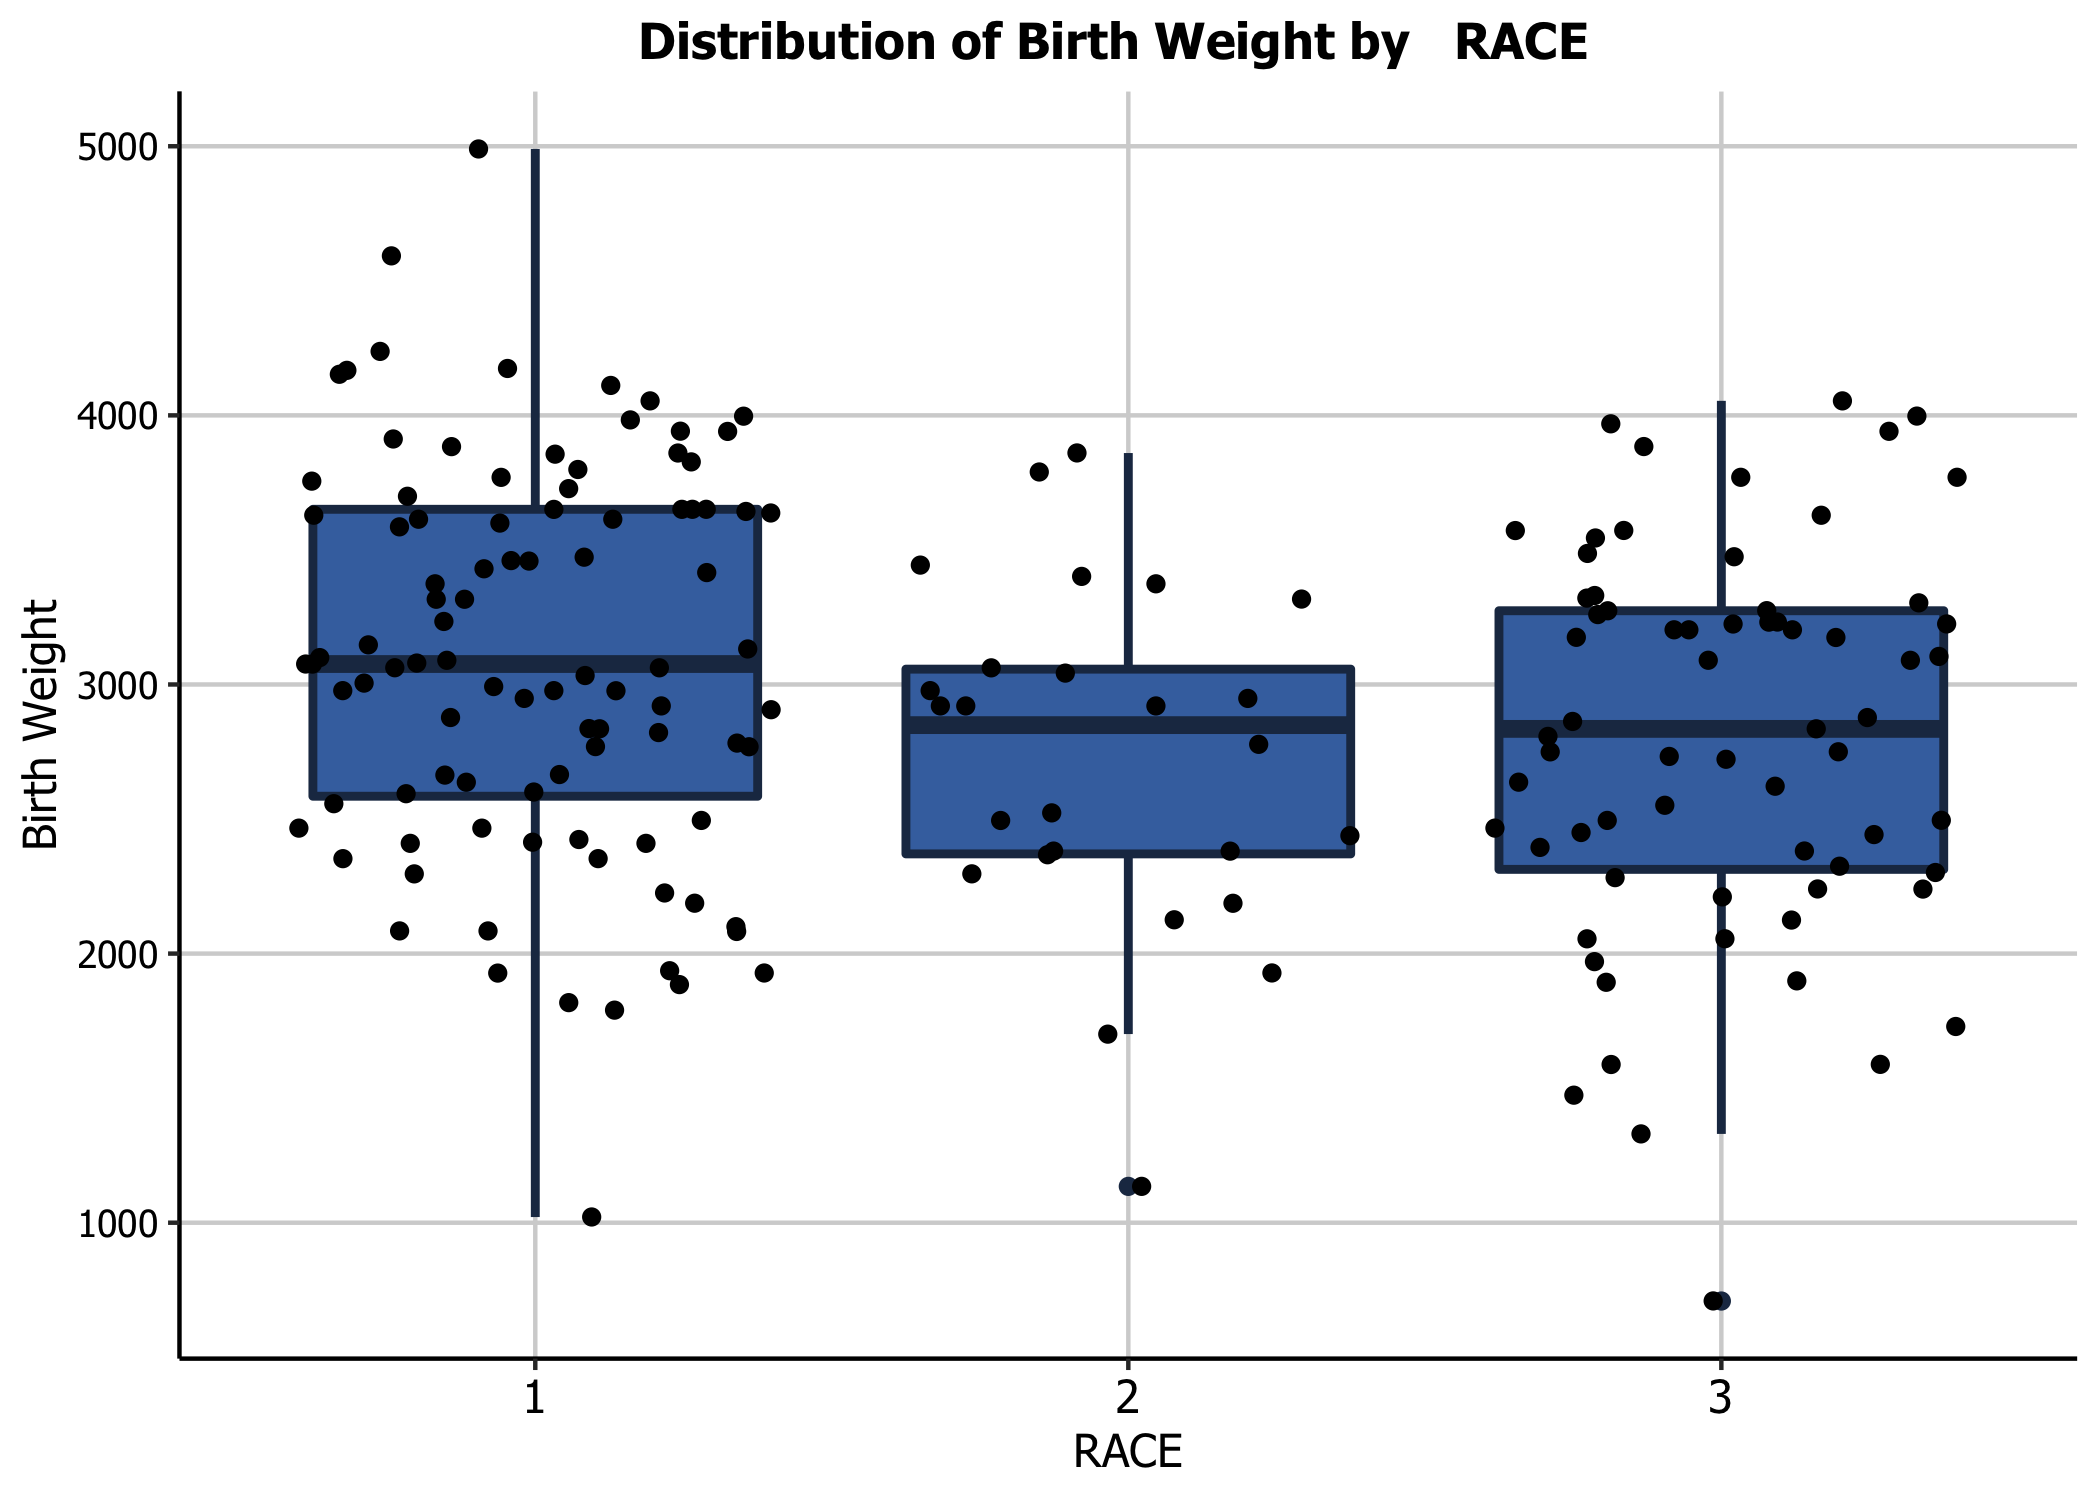
\includegraphics[width=\textwidth]{Images/RACE.png}
            \label{fig:BWTvsRACE}
        \end{subfigure}
        
        \hfill
        
        \begin{subfigure}[b]{0.4\textwidth}   
            \centering 
            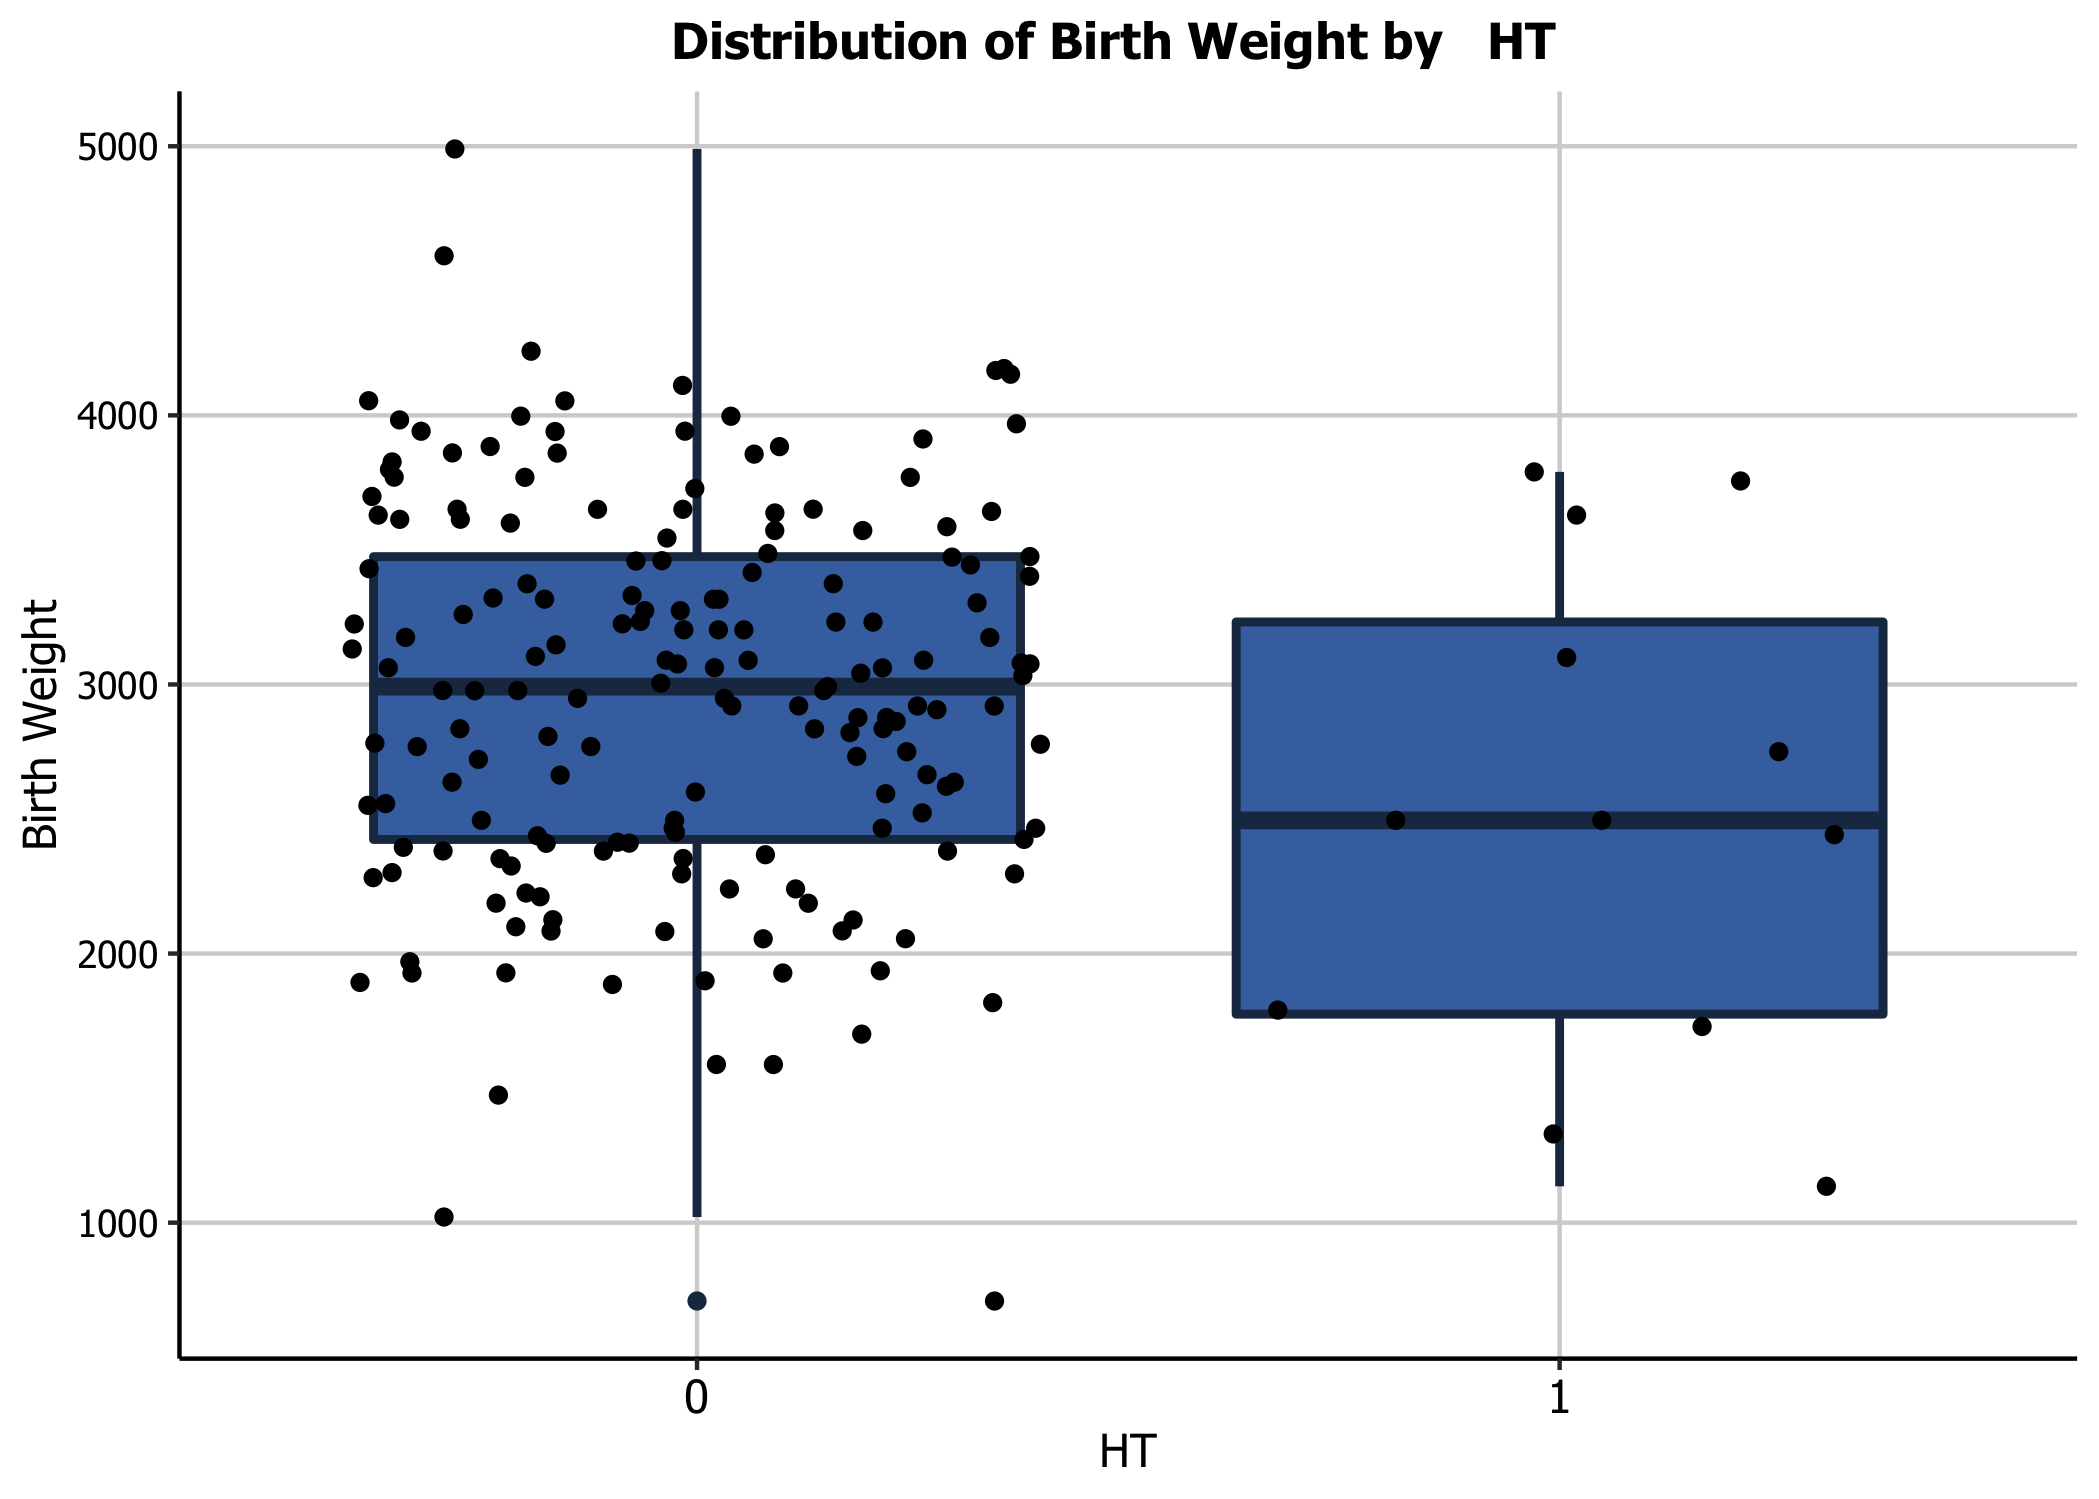
\includegraphics[width=\linewidth]{Images/HT.png}
            \label{fig:BWTvsHT}
        \end{subfigure}
        \quad
        \begin{subfigure}[b]{0.4\textwidth}   
            \centering 
            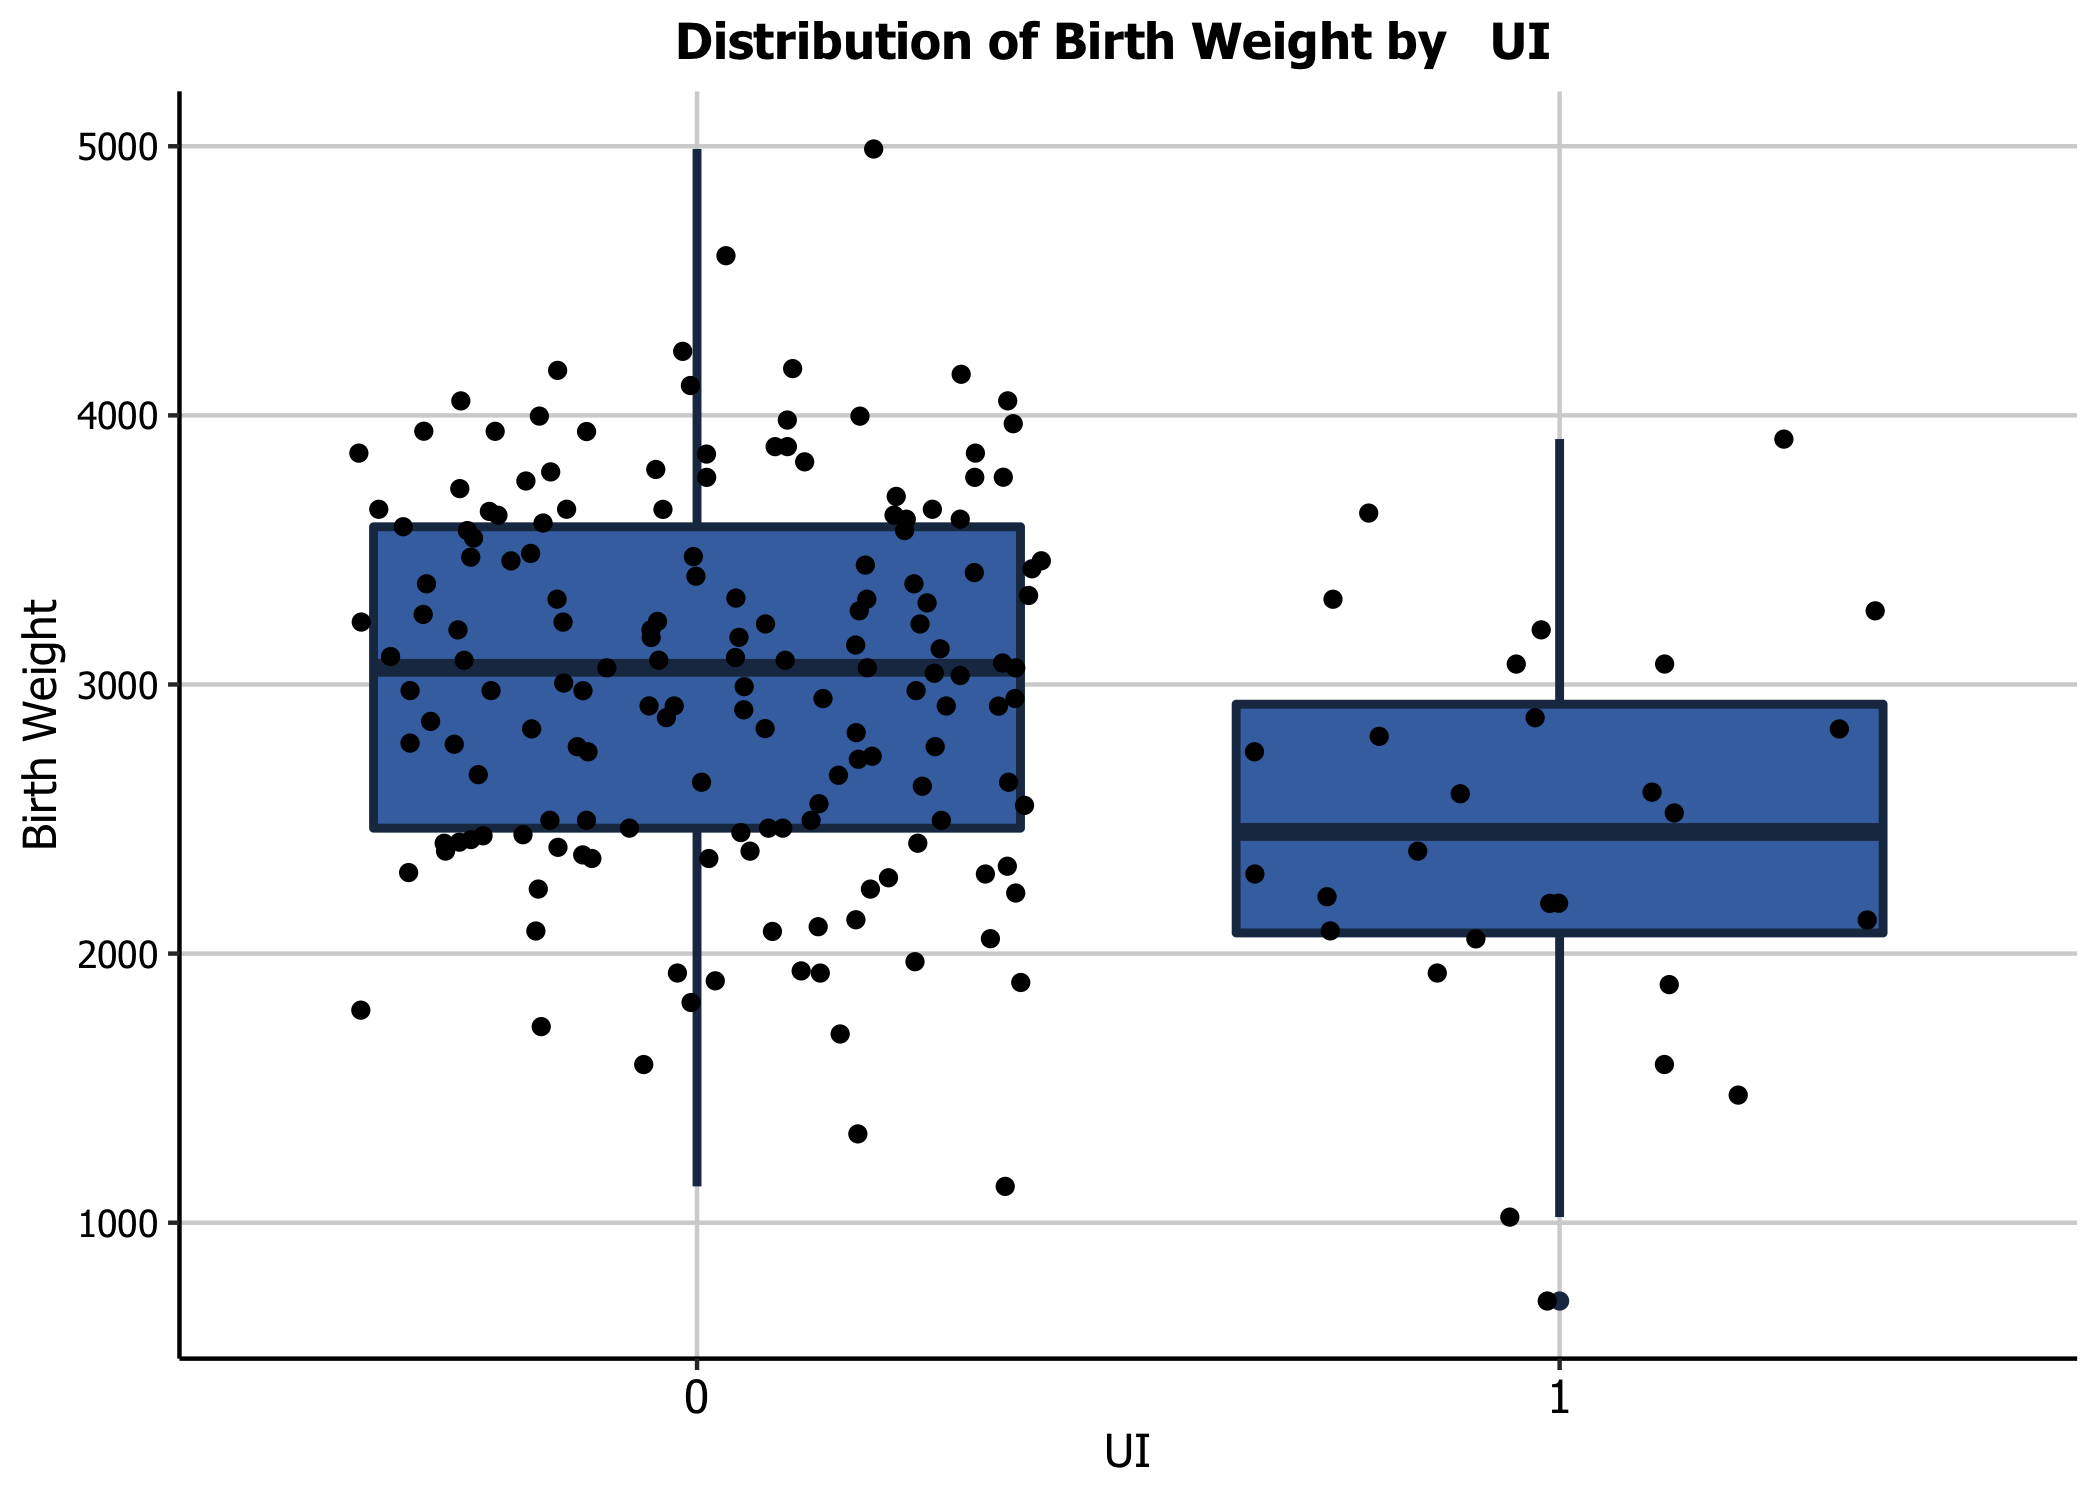
\includegraphics[width=\linewidth]{Images/UI.png}
            \label{fig:BWTvsUI}
        \end{subfigure}
        \caption[ The average and standard deviation of critical parameters ]
        {\small Box plots for each of the non-continuous variables against birth weight.} 
        \label{fig:Non-continuous}
    \end{figure}

\textbf{BWT vs RACE:} The mean birth weight for black women and the 'other' group are both slightly lower than for white women (~200 g). These results are consistent with the obstetrical literature.

\textbf{BWT vs SMOKE:} Note that the mean birth weight for infants of smokers is ~2700g and the mean for infants of non-smokers is ~3100g. There is a clear negative association between maternal smoking and birth weight in the dataset.

\textbf{BWT vs HT:} The mean infant birth weight for pregnant women with hypertension is lower than the mean infant birth weight of those without hypertension. It is important to note that only a few women in our dataset have a history of hypertension, nonetheless the association is consistent with the literature.\cite{HT-LBW}\cite{InducedHT}\cite{HTRace}

\textbf{BWT vs UI:} Note the 600g difference in mean birth weight between women without UI (3100g) and those with UI (2500g). This is again consistent with the literature and suggests that UI should be strongly considered as a main effect in the candidate models.

\subsection{Interactions Between Sets of Variables} \label{ExploratoryInteractions}
Drawing from the interactions found in the obstetrical literature, we investigate whether these interactions are also relevant in our dataset. Speculative investigations of different interactions were also performed and these interactions are visualised in the plots below.

\vspace{0.5cm}
\begin{figure}[!htb]
        \centering
        \begin{subfigure}[b]{0.4\textwidth}
            \centering
            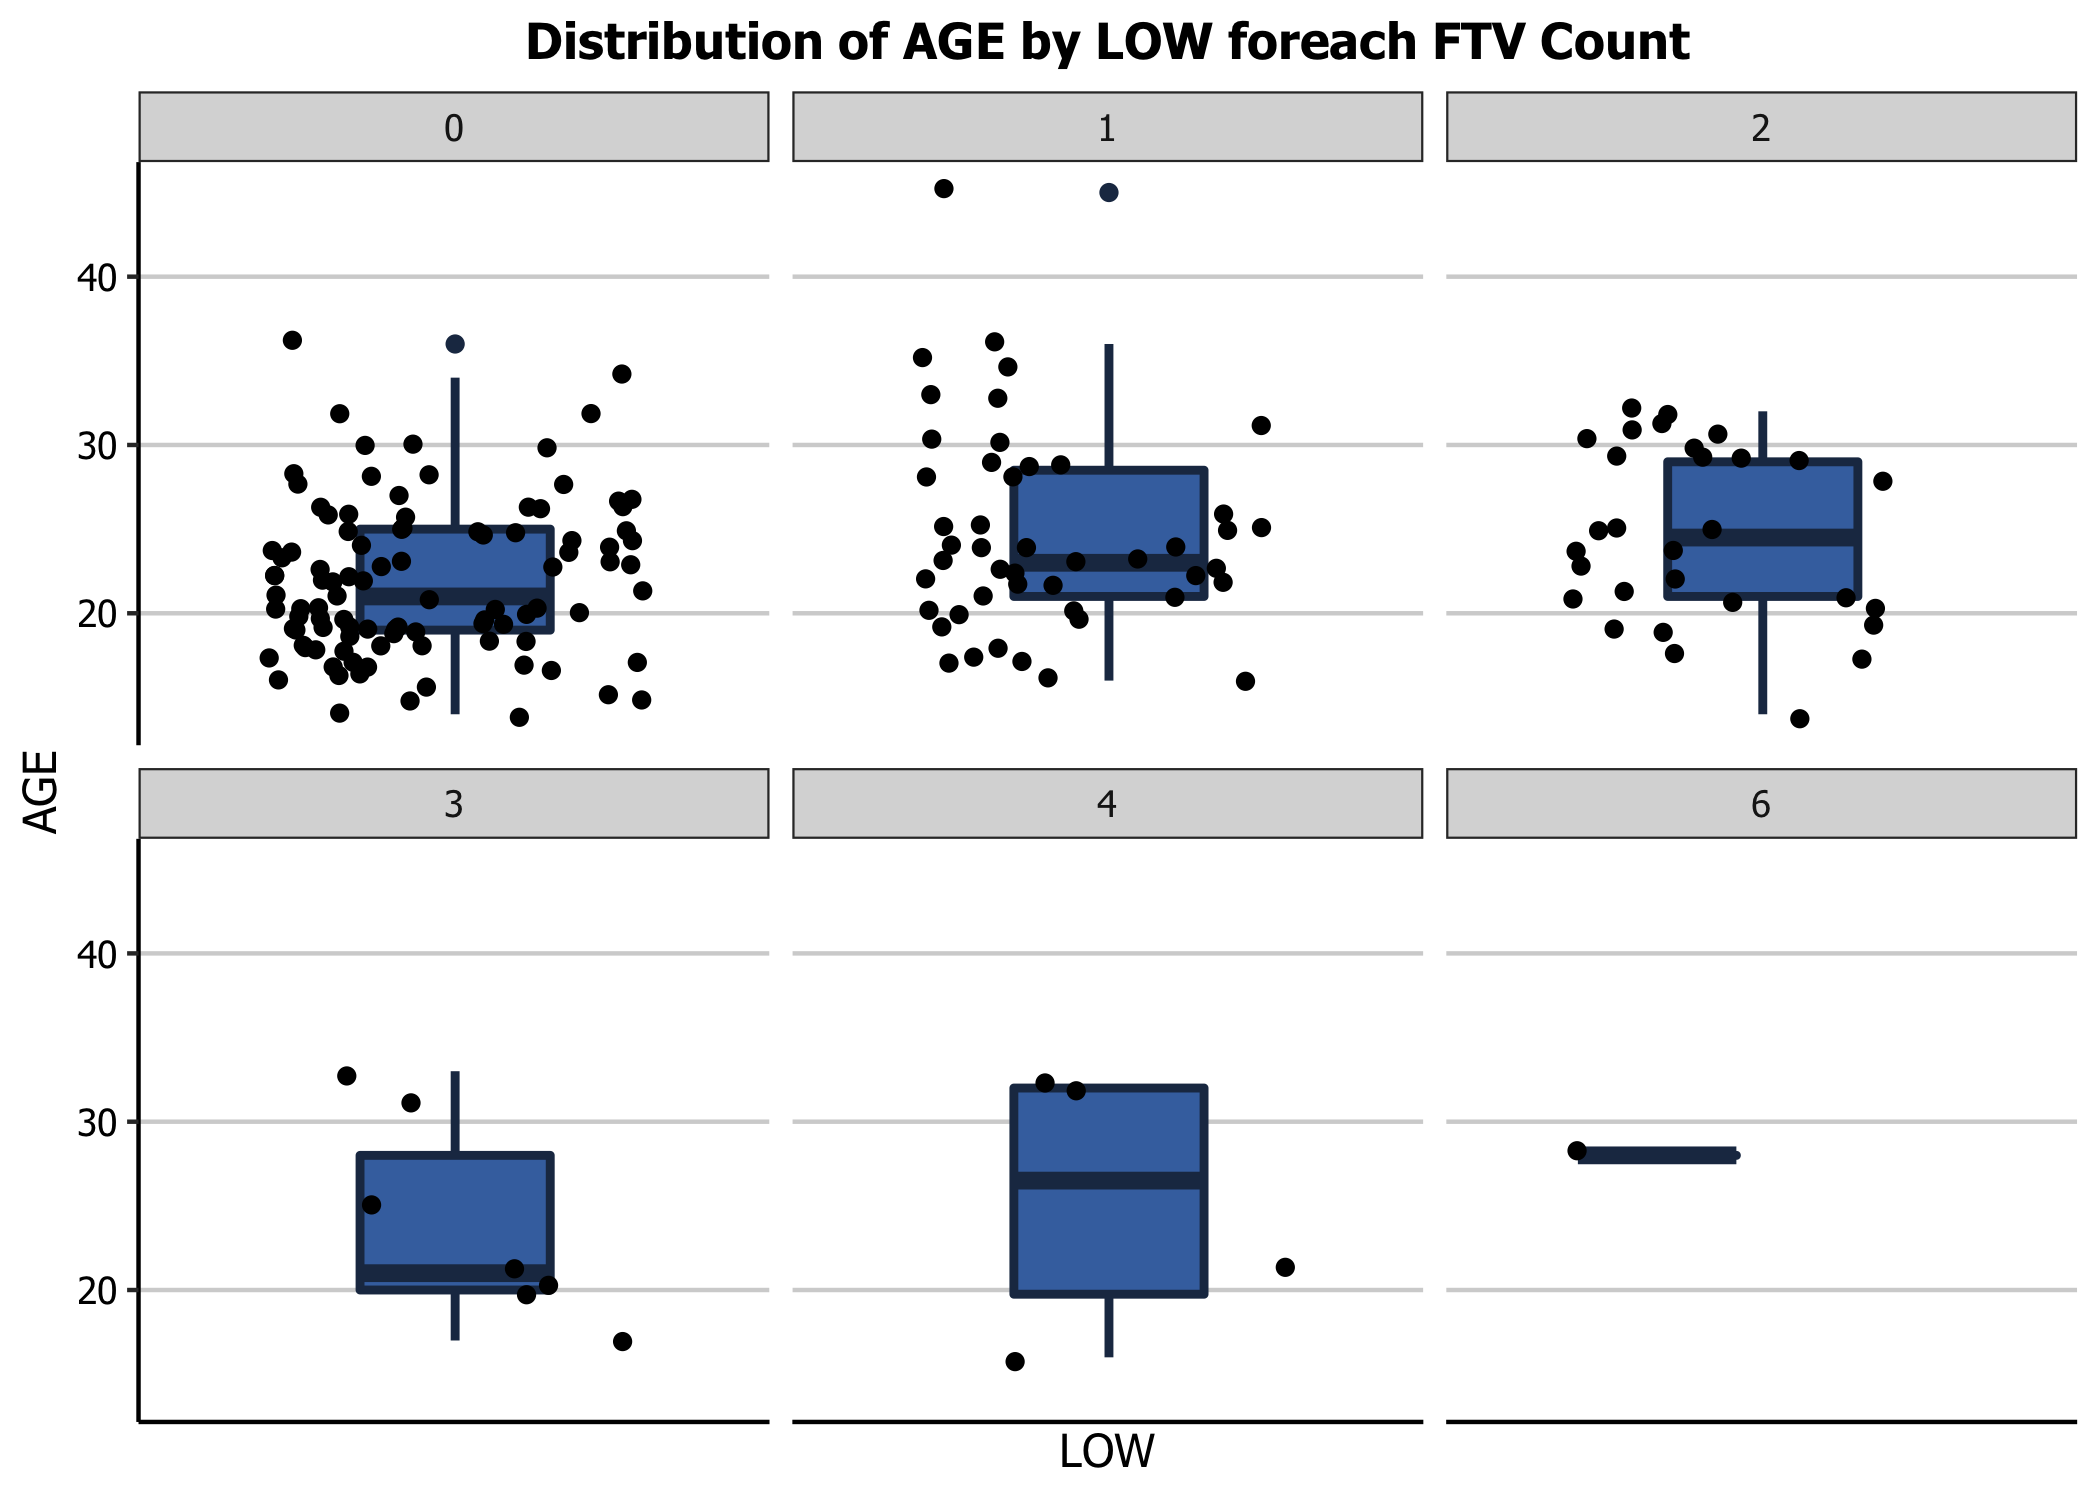
\includegraphics[width=\textwidth]{Images/AgeFtv.png}
        \end{subfigure}
        \quad
        \begin{subfigure}[b]{0.4\textwidth}  
            \centering 
            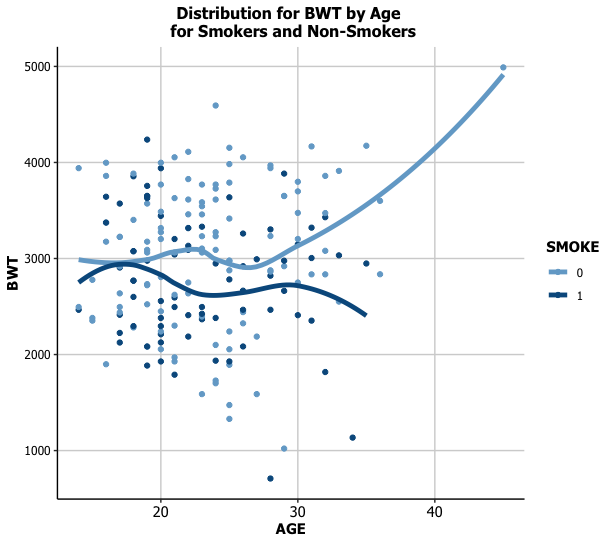
\includegraphics[width=\textwidth, height=4.4cm]{Images/AgevsSmoke_Magda.png}
        \end{subfigure}
        
        \hfill
        
        \begin{subfigure}[b]{0.4\textwidth}   
            \centering 
            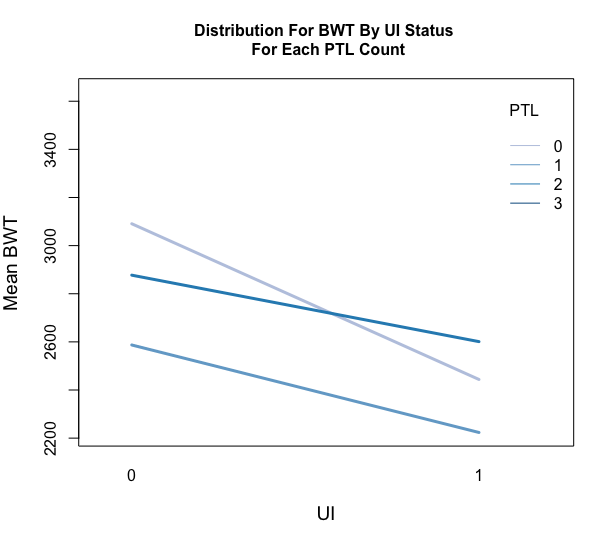
\includegraphics[width=\linewidth]{Images/PtlvsUi_Magda.png}
        \end{subfigure}
        \quad
        \begin{subfigure}[b]{0.4\textwidth}   
            \centering 
            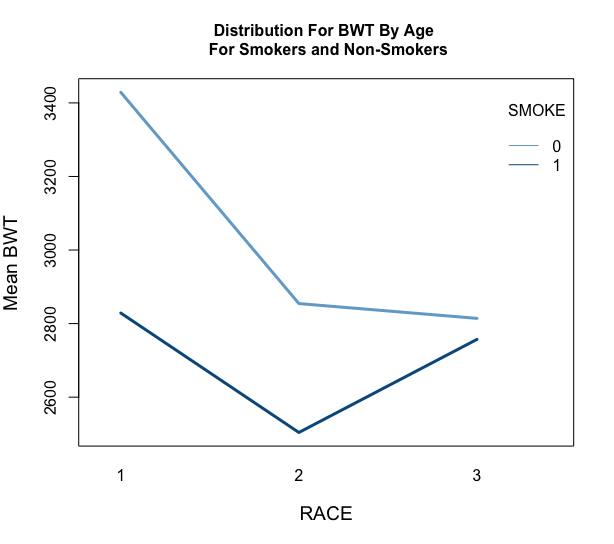
\includegraphics[width=\linewidth]{Images/RacevsSmoke_Magda.png}
        \end{subfigure}
        \caption[ The average and standard deviation of critical parameters ]
        {\small Box plots for each of the significant interaction terms.} 
        \label{fig:interactionplots}
    \end{figure}

\begin{itemize}
    \item \textbf{AGE/FTV -} There is a clear difference in the mean birth weight both within and between FTV groups. This suggests that the number of physician visits might have a varying effect birth weight depending on maternal age. It is important to note, however, that there are few data points in FTV groups 3 and 4, and only one in group 6. Care is therefore needed when extrapolating the significance of this interaction term, due to the limited number of data points.
    
    \item \textbf{RACE/SMOKE -} This plot shows that the effect of smoking on birth weight is dependent on race. This is consistent with the obstetrical literature and gives us reason to include it in our candidate models.
    
    \item \textbf{UI/PTL -} From this plot, it appears the effect of UI on birth weight is reduced for women with more pre-term labours. This gives us reason to include it in our models and see if it is statistically significant. This details of how exactly these variables interact will be discussed in section \ref{sec:interpretation}.
    
    \item \textbf{AGE/SMOKE -} The plot shows the data points for smokers vs non-smokers, along with the mean birth weight at each age. As the lines are not parallel, there is evidence of some interaction.
    
\end{itemize}

\section{Question 1}
The four variables which are considered the most clinically important are AGE, LWT, RACE, and FTV. Using these variables, a model building exercise is carried out using AIC and AIC weights to determine the model that best fits the data.

\subsection{Model Building} \label{BuildingOne}
There is a trade-off between accuracy and interpretability when deciding on the number and order of interaction terms to include in these models. Due to this fact, only a small number of first-order interaction terms are included in the candidate models. The interaction terms included in the candidate model are the significant interactions determined by the literature review and exploratory analysis (see sections \ref{literatureInterations} and \ref{ExploratoryInteractions}). The principle of constructing hierarchical models also dictates that if an interaction term is included, the constitutive main effect variables should also be included.

First a model is constructed with the main effects only:

\begin{equation}
    \text{RACE + FTV + AGE + LWT}
\end{equation}

Secondly, a model with all interaction terms:

\begin{equation}
\label{eq:FullModel}
    \text{RACE + FTV + AGE + LWT + LWT/FTV + AGE/FTV}
\end{equation}

Then models with each singular interaction term:

\begin{equation}
    \text{RACE + FTV + AGE + LWT + AGE/FTV}
\end{equation}

\begin{equation}
    \text{RACE + FTV + AGE + LWT + LWT/FTV}
\end{equation}

The final two candidate models retain $AGE/FTV$ as an interaction term because it is highly suggested by the exploratory analysis that it is significant. These models examine the effect of adding both LWT and RACE individually as main effects.

\begin{equation}
    \text{RACE + FTV + AGE + AGE/FTV}
\end{equation}

\begin{equation} \label{eq:bestmodelone}
    \text{FTV + AGE + LWT + AGE/FTV}
\end{equation}

\subsection{Comparing the Models}
The models are evaluated against each other using a modification of the Akaike Information Criterion (AIC). When the sample size is small, there is a substantial probability that AIC will select models that have too many parameters - AIC will overfit. To address overfitting, AICc is used: AICc is AIC with a correction for small sample sizes: 

\begin{equation}
    \text{AICc} = \text{AIC} + \frac{2k^2 + 2k}{n-k-1}
\end{equation}

where $n$ denotes the sample size and $k$ is the number of parameters in the model. Note that as $n\to\infty$, the penalty term tends to $0$ and AICc converges to AIC. The results for each of the models are shown below.

\vspace{0.3cm}
\renewcommand\arraystretch{1.2}
\begin{table}[hbt!]
    \centering
    \begin{tabular}[t]{p{8cm}ccc}
        \toprule
        Model & AICc Score & $\Delta$ AICc & AICc Weight \\
        \midrule
        \rowcolor{blue!15}
        \small{$AGE+FTV+LWT+AGE/FTV$} & 225.70 & 0.00 & 0.57 \\
        \small{$AGE+RACE+FTV+LWT+AGE/FTV$} & 227.24 & 1.54 & 0.26 \\
        \small{$AGE+RACE+FTV+LWT+AGE/FTV+LWT/FTV$} & 228.79 & 3.09 & 0.12 \\
        \small{$AGE+RACE+FTV+AGE/FTV$} & 231.34 & 5.65 & 0.03 \\
        \small{$AGE+RACE+FTV+LWT$} & 235.03 & 9.34 & 0.01 \\
        \small{$AGE+RACE+FTV+LWT+LWT/FTV$} & 236.64 & 10.94 & 0.00 \\
        \bottomrule
    \end{tabular}
    \caption{Comparison of candidate models using AICc. The best performing model is highlighted.}
    \label{tab:ModelOneComparison}
\end{table}%

Based on the AICc weights, we determine that the best model is given by equation \ref{eq:bestmodelone}. The final model with coefficients and intercept is given by:

\begin{equation} \label{eq:finalmodel}
    \mathbb{E}(\text{LOW}) = -\textcolor{purple}{0.166} + \textcolor{purple}{0.0658}\text{AGE} - \textcolor{purple}{2.844}\text{FTV} -\textcolor{purple}{0.0155} \text{LWT} - \textcolor{purple}{0.131} \text{AGE/FTV}
\end{equation}

A final model was also constructed using the backward elimination procedure. Starting with the full model given by equation \ref{eq:FullModel}, the variable with the highest p-value controlling the type 1 error at $\alpha = 0.1$ was iteratively removed. Both $FTV/LWT$ and $RACE$ were removed using this procedure, resulting in the same model given in the equation above.

Each of the AICc, backward elimination, and stepwise selection procedures give the same final model. The AICc criterion for each of these is given below.

\renewcommand\arraystretch{1.2}
\begin{table}[hbt!]
    \centering
    \begin{tabular}[t]{lll}
        \toprule
        Procedure & Model & AICc \\
        \midrule
        Using AICc & \small{$LOW\thicksim AGE+FTV+LWT+AGE/LWT$} & 225.70 \\
        Backward Selection & \small{$LOW\thicksim AGE+FTV+LWT+AGE/LWT$} & 225.37 \\
        Stepwise selection & \small{$LOW\thicksim AGE+FTV+LWT+AGE/LWT$} & 225.37 \\
        \bottomrule
    \end{tabular}
    \caption{Comparison of AICc scores using the different model selection methods.}
    \label{tab:comparison-4variables}
\end{table}%

\section{Question Two}
The set of potential predictive variables is expanded to include UI, HT, PTL, and SMOKE. Using the same procedures outlined in \ref{BuildingOne}, candidate models are chosen and then compared. The final model is then interpreted in terms of the coefficients and odds ratios.

\subsection{Model Building} \label{BuildingTwo}
The candidate models were constructed according to the principles outlined in section \ref{BuildingOne}. First constructing a model with main effects only and one full model with all relevant interactions determined by the exploratory analysis and literature review. Then different models were constructed to isolate the effect of different main effect and interaction terms. These models are shown in table \ref{tab:ModelTwoComparison}.

\subsection{Comparing the Models}
The models are evaluated against each other using the modified Akaike Information Criterion (AICc). The results for the models are shown below. In total, 11 candidate models were compared, only a subset of which are shown here, as they are interesting to compare. 

\renewcommand\arraystretch{1.2}
\begin{table}[ht]
    \centering
    \begin{tabular}[t]{lccc}
        \toprule
        Model & AICc Score & $\Delta$ AICc & AICc Weight \\
        \midrule
        \rowcolor{blue!15}
        \small{$LWT+HT+SMOKE+PTL/UI+AGE/FTV$} & 211.53 & 0.00 & 0.30 \\
        \small{$LWT+HT+SMOKE+RACE+AGE/FTV+PTL/UI$} & 212.24 & 0.71 & 0.21 \\
        \small{$LWT+HT+PTL/UI+AGE/FTV$} & 212.30 & 0.77 & 0.21 \\
        \small{$FTV+LWT+HT+SMOKE+RACE+PTL/UI$} & 220.71 & 9.18 & 0.00 \\
        \small{$AGE+FTV+LWT+HT+SMOKE+RACE+PTL/UI$} & 221.96 & 10.43 & 0.00 \\
        \bottomrule
    \end{tabular}
    % \captionsetup{width=.69\linewidth}
    \caption{Comparison of a subset of the candidate models using AICc. The best performing model is highlighted.}
    \label{tab:ModelTwoComparison}
\end{table}%

The best performing model does not include RACE as a main effect, and contains only AGE/FTV and PTL/UI as interaction terms. The importance of these interaction terms is clear as they are present in each of the best performing models. Removing AGE as a main effect or removing AGE/FTV as an interaction term significantly inhibits the performance of the model. It is also interesting to note that model 2 and 3 perform similarly, even though model 3 does not have SMOKE or RACE as main effects. We can interpret this as the information gained from these two variables is offset by the complexity penalty included in the AICc formula.

A summary of the models and AICc scores for backward selection, stepwise selection, and AICc procedures is given below below. Note that they all result in the same final model, although both backward and stepwise selection have better AICc scores.

\vspace{0.3cm}
\renewcommand\arraystretch{1.2}
\begin{table}[ht]
    \centering
    \begin{tabular}[t]{lll}
        \toprule
        Procedure & Model & AICc \\
        \midrule
        Using AICc & $LOW\thicksim AGE/FTV+PTL/UI+LWT+HT+SMOKE$ & 211.53 \\
        Backward Selection & $LOW\thicksim AGE/FTV+PTL/UI+LWT+HT+SMOKE$ & 210.3 \\
        Stepwise selection & $LOW\thicksim AGE/FTV+PTL/UI+LWT+HT+SMOKE$ & 210.3 \\
        \bottomrule
    \end{tabular}
    \caption{Comparison of AICc scores using the different model selection methods.}
    \label{tab:comparison-8variables}
\end{table}%

The final model is given by:

\vspace{-0.5cm}
\begin{equation}
    \begin{split}
    \small{LOW\thicksim \textcolor{purple}{0.0721} \text{AGE} + \textcolor{purple}{3.4535} \text{FTV} + \textcolor{purple}{1.1812} \text{PTL} + \textcolor{purple}{1.5861} \text{UI} + \textcolor{purple}{0.6389} \text{SMOKE}} \\
    \small{+ \textcolor{purple}{1.8637} \text{HT} - \textcolor{purple}{0.0155} \text{LWT} - \textcolor{purple}{0.1551} \text{AGE/FTV} -\textcolor{purple}{1.6058} \text{PTL/UI}}
    \end{split}
\end{equation}

\subsection{Interpreting the Final Model} \label{sec:interpretation}
The final model can be interpreted in terms of odds ratios. The odds ratios are given $e^{\beta_i}$, where $\beta_i$ is the coefficient for the $i^{\text{th}}$ parameter. It is important to note that any main effect variables which are present in an interaction must be interpreted in terms of that interaction. Those main effect terms which are not present in interactions, along with their respective odds ratios, are given below.

% \vspace{0.3cm}
\renewcommand\arraystretch{1.2}
\begin{table}[ht]
    \centering
    \begin{tabular}[t]{lccc}
        \toprule
        & SMOKE & HT & LWT \\
        \midrule
        $\beta_i$ & 0.6389 & 1.8637 & -0.0155 \\
        $e^\beta_i$ & 1.89 & 6.44 & 0.98 \\
        \bottomrule
    \end{tabular}
    \caption{Coefficients and odds ratios for main-effects in the final model.}
    \label{tab:main-effect-odds}
\end{table}%

How are these odds ratios interpreted? For example, SMOKE has an odds ratio of 1.89, which means that the odds of a low birth weight if the mother smokes during pregnancy are 1.89 times larger if the mother does not smoke. For continuous predictor variables such as LWT, the odds ratio gives the change in the likelihood of a low birth weight per unit increase in that variable. The odds ratio for LWT is 0.985, which means that the odds of a low birth weight decrease by 1.5\% with every unit increase in LWT. To use a more illustrative example, a ten pound increase in LWT is associated with a $1-\exp(10-0.00155) = 14\%$ decrease in the likelihood of a low-weight birth. Of the significant covariates not involved in an interaction, a history of hypertension has the strongest effect on the likelihood of a low weight birth - which is consistent with the obstetrical literature.

As AGE/FTV and PTL/UI interact significantly in the model, the effect of each consitutive main-effect variable on the likelihood of a low birth weight must be interpreted with its paired variable in mind. The strength of one variable’s effect on the likelihood of a low birth weight is dependent on the value of the other. The interaction between AGE and FTV is an illustrative one. To better understand the AGE/FTV interaction, one can consider three mothers, at three different ages (14, 25, and 45), and calculate the respective odds ratios. The odds ratios are calculated using the following formula:

\begin{equation}
    OR = exp\:(Odds_{FTV} - Odds_{AGE/FTV}\cdot AGE) = exp\:(3.45 - 0.155\cdot AGE)
\end{equation}

for $AGE = 14$ this gives,

\begin{equation}
    OR = exp\:(3.45 - 0.155\cdot 14) = 3.6
\end{equation}

This means that the likelihood of a low birth weight for mothers aged 14 is 3.6 times larger if FTV is increased by 1.
Using the same method to calculate the odds ratio for women aged 25 and 45 gives odds ratios of 0.655 and and 0.029, respectively. The scientific insight gained from this is that the effectiveness of physician visits in reducing the likelihood of low birth weights increases as age increases.

For the PTL/UI interaction, it is interesting to calculate the bidirectional effects of this interaction. The formulae for calculating the odds ratios are given by

\begin{equation}
    OR = exp\:(Odds_{PTL} - Odds_{UI/PTL}\cdot UI) = exp\:(1.181 - 1.605\cdot UI)
\end{equation}

\begin{equation}
    OR = exp\:(Odds_{UI} - Odds_{UI/PTL}\cdot PTL) = exp\:(1.586 - 0.1605\cdot PTL)
\end{equation}

Using these equations it was determined that the odds a low birth weight for a mother with no history of UI is 3.26 times larger when the number of PTLs increases by one. For a mother with no history of UI, the odds are 0.653 times lower when the number of PTLs increases by one. This shows that the effect of increasing PTL is significantly weaker in mothers with a history of UI. 

In the other direction, these equations can be used to examine the effect the UI has on the likelihood of a low birth weight, depending on the number of previous pre-term labours. For example, when PTL is 0, the odds of having a newborn with LBW if the mother has UI is 4.88 times larger than the odds of having a newborn with LBW if the mother doesn’t have UI. When PTL is 2, the odds of having a newborn with LBW if the mother has UI is 0.1968 times the odds of having a newborn with LBW if the mother doesn’t have UI.

\newpage
\section{Scientific Insight}
In brief, the odds ratios derived from the final model indicate that both smoking during pregnancy and a history of hypertension increase the likelihood of a low birth weight, while an increase in the maternal weight before pregnancy slightly reduces the likelihood. The model also indicates that visits to the physician are most effective in older mothers. 


\section{Limitations}
The majority of the limitations faced in this project are a result of issues with the size and nature of the dataset. Due to the limited size, there were some categories with little data. For example, there was only one woman who had visited the physician six times, which heavily impacted interaction terms containing FTV. Extrapolating and making inferences from small sample sizes such as this is dubious, and this ultimately affected our confidence in the final models and their interpretations.

Some of the covariates in the dataset could be improved, which would lead to more representative models. For example the BMI of the mother at her last menstrual period is a far superior metric than her weight at her last menstrual period. Furthermore, as established by other studies, race effectively serves as a proxy variable for other sociodemographic, behavioural, and cultural variables. A model built on a dataset which contains these variables would be easier to interpret.

Low birth weight has two primary causes: pre-term birth and intrauterine growth restriction (IUTG). The covariates used in this study affect both pre-term birth and IUTG differently. For example, smoking has a much larger effect on the likelihood of IUTG than on pre-term birth. If data had been collected on the age of the fetus in weeks, it would be possible to distinguish between the two phenomena and to construct models accordingly. Clinically, the distinction between these two phenomena is critical as each requires a different course of action. An inability to distinguish between these two phenomena brings into question whether any predictions from these models are clinically actionable.

\subsection*{How confident do we feel about the selected models?}
An extensive literature review was conducted and exploratory analysis performed before approaching this dataset to ensure that predictors or interactions were not being chosen blindly according to the significance indicated by the GLM. The final models offer specific insight into the degree to which the covariates influence the likelihood of a low birth weight. Furthermore, the models give insight into how these covariates interact with each other to affect this likelihood.

Our confidence in these models is buttressed by the fact that multiple model building procedures resulted in the same final models. While we are aware there is no perfect model, we believe that the final two models chosen represent the ‘best case scenarios’ of the models that could be generated, and that they give a sensible binary prediction of low birth weight given the scope of the dataset available to us.

Confidence in these models could be improved with additional data and testing. This data would help to validate the final coefficients and resolve issues relating to the sparsity of the data. Additionally, a larger dataset would allow us to partition the dataset into a training, test, and validation set, which would allow us to investigate whether the model generalises well to a larger population. Lastly, comparison to models that perform regression for continuous birth weight data may help us to identify any flaws in our model that stem from converting continuous birth weights into binary categorisation.